\subsection{Overview License Verification}
\begin{itemize}
  \item looks like solution
  \item does not prevent from copying, but implements mechanism independent
  \item all work by talking to other instance, evaluating result
  \item based on yes/no answer
  \item google started, others followed since they want developers to come to store
  \item since dex, can be decompiled and analyses then attacked, even cracking solutions available for the big players
  \item developer has to decide between reach and security, unknown stores are not likely to be attacked but developer cannot sell apps that well, but if the app attracts attention, even these unknown stores will be cracked
\end{itemize}

\subsection{Abstraction} \label{section:license-abstraction}
\begin{figure}[h]
    \centering
    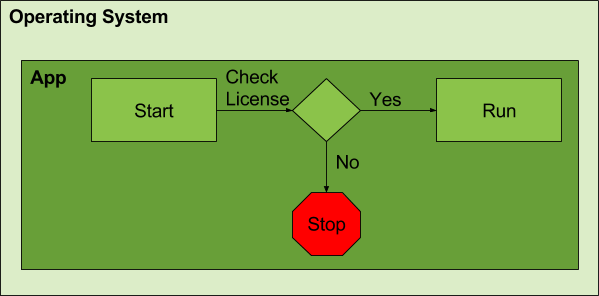
\includegraphics[width=0.8\textwidth]{data/verificationNow.png}
    \caption{Abstraction of the current license verification mechanism. The library is represented by (1)}
    \label{fig:verificationNow}
\end{figure}
